\documentclass[../DefinizioneDiProdotto.tex]{subfiles}
\begin{document}
		\section{Specifica delle componenti}
			\subsection{SWEDesigner}
				I package contenuti al suo interno sono:
				\begin{itemize}
					\item SWEDesigner::Client;
					\item SWEDesigner::Server.
				\end{itemize}
				Questo package non contiene delle classi.
			\subsection{SWEDesigner::Client}
				% IMMAGINE ARCHITETTURA CLIENT GENERALE
				\begin{figure}[H]\label{fig:ClientSubsystem}
					\centering
					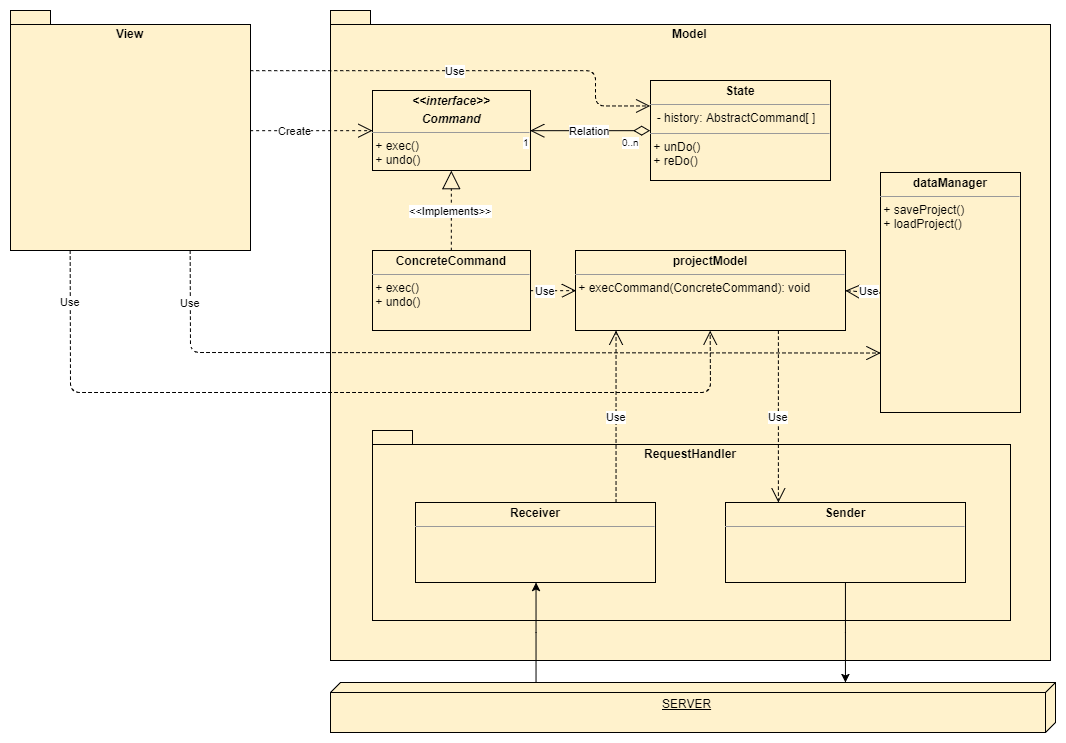
\includegraphics[scale=0.46]{Immagini/DiagrammaArchitettura/ClientSubsystem.png}
					\caption{Architettura del client}
				\end{figure}
				I package contenuti al suo interno sono:
				\begin{itemize}
					\item SWEDesigner::Client::Model;
					\item SWEDesigner::Client::View.
				\end{itemize}
				Questo package non contiene delle classi.
			\subsection{SWEDesigner::Client::Model}
				\hypertarget{SWEDesigner::Client::Model}
				I package contenuti al suo interno sono:
				\begin{itemize}
					\item SWEDesigner::Client::Model::Items.
				\end{itemize}
				Le classi contenute al suo interno verranno elencate qui di seguito.

				\subsubsection{SWEDesigner::Client::Model::DataManager}
				\hypertarget{SWEDesigner::Client::Model::DataManager}{}
					\begin{itemize}
						\item \textbf{Tipo}: \emph{Classe statica};
						\item \textbf{Descrizione}: Si occupa della persistenza dei dati, in particolare del salvataggio su file system locale del progetto già esistente.\\;
						\item \textbf{Metodi}:
						\begin{itemize}
							\item \emph{newProject(): void} \\
							Dopo aver chiesto conferma all'utente, crea un nuovo progetto sovrascrivendo quello correntemente aperto; \\
							\item \emph{openProject(): void} \\
							Legge un file JSON e ne salva il contenuto in project e nel projectModel come progetto attualmente aperto; \\
							\item \emph{save(fileName: String): void} \\
							Salva i dati del progetto, li converte in formato JSON e avvia la procedura di download in locale del browser; \\
							\textbf{Parametri}:
							\begin{itemize}
								\item \emph{fileName: String}
								Nome del file generato da scaricare; \\
							\end{itemize}
							\item \emph{saveAs(): void}\\
							Estrae la stringa inserita dall'utente nella schermata per il salvataggio con nome e invoca la il metodo per il salvataggio del progetto corrente in un file con il nome desiderato; \\
						\end{itemize}
						\item \textbf{Relazioni con le altre classi}:
						\begin{itemize}
							\item OUT \hyperlink{SWEDesigner::Client::Model::ProjectModel}{\emph{SWEDesigner::Client::Model::ProjectModel}}: si occupa di gestire la parte logica dell'editor;
							\item OUT \hyperlink{SWEDesigner::Client::Model::Project}{\emph{SWEDesigner::Client::Model::Project}}: si occupa di gestire gli elementi contenuti nel diagramma.
						\end{itemize}
					\end{itemize}

				\subsubsection{SWEDesigner::Client::Model::ProjectModel}
				\hypertarget{SWEDesigner::Client::Model::ProjectModel}{}
					% IMMAGINE ARCHITETTURA MAINMODEL
					\begin{figure}[H]\label{fig:Model}
						\centering
						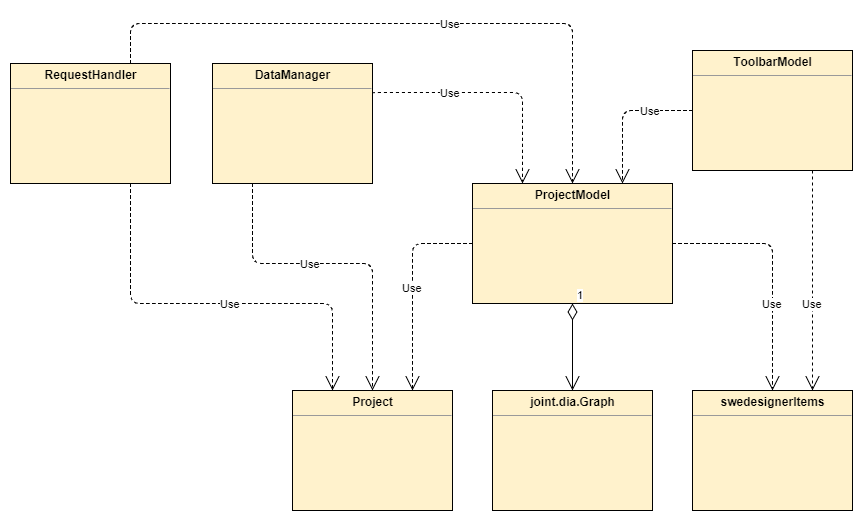
\includegraphics[scale=0.46]{Immagini/DiagrammaArchitettura/MainModel.png}
						\caption{Architettura di Model}
					\end{figure}

					\begin{itemize}
						\item \textbf{Tipo}: \emph{Classe};
						\item \textbf{Descrizione}: Model del progetto corrente. Si occupa di gestire il graph (joint.dia.Graph) e tutti gli eventi ad esso associati;
						\item \textbf{Padre}: \emph{Backbone.model};
						\item \textbf{Attributi}:
						\begin{itemize}
							\item \emph{currentDiagram: String} \\
							L'id del diagramma correntemente caricato nel graph (null se è il diagramma dei package); \\
							\item \emph{currentDiagramType: String} \\
							Il tipo del diagramma correntemente caricato nel graph ("packageDiagram", "classDiagram" o "bubbleDiagram"); \\
							\item \emph{graph: joint.dia.Graph} \\
							Il model dell'area di disegno associata al paper della \hyperlink{SWEDesigner::Client::View::ProjectView}{\emph{SWEDesigner::Client::View::ProjectView}}; \\
							\item \emph{itemToBeAdded: String} \\
							Salvataggio temporaneo dell'elemento da aggiungere al graph corrente; \\
						\end{itemize}
						\item \textbf{Metodi}:
						\begin{itemize}
							\item \emph{addItem(item: Object): void} \\
							Salva in itemToBeAdded l'elemento passato in input che è un oggetto di Swedesigner::Client::Model::Items; \\
								\textbf{Parametri}:
								\begin{itemize}
									\item \emph{item: Object}
									Elemento del diagramma; \\
								\end{itemize}
							\item \emph{addItemToGraph(): void} \\
							Aggiunge un elemento al grafo del diagramma corrente; \\
							\item \emph{changedPosition(graph: joint.dia.Graph, cell: joint.dia.Cell, newPosition: Object, opt: Object): void} \\
							Gestisce la traslazione di un elemento selezionato nel grafo; \\
								\textbf{Parametri}:
								\begin{itemize}
									\item \emph{graph: joint.dia.Graph}
									Grafo del diagramma corrente; \\
									\item \emph{cell: joint.dia.Cell}
									Elemento correntemente selezionato; \\
									\item \emph{newPosition: Object}
									Posizione attuale dell'oggetto nel grafo; \\
									\item \emph{opt: Object}
									Traslazione dell'oggetto dalla posizione iniziale alla posizione "newPosition"; \\
								\end{itemize}
							\item \emph{deleteCell(): void} \\
							Rimuove un elemento dal grafo eliminando anche gli eventuali diagrammi derivati (classi o bubble); \\
							\item \emph{deleteOperation(): void} \\
							Rimuove un'operazione ed eventualmente anche il diagramma delle bubble associato; \\
							\item \emph{getCellFromId(cellId: String): void} \\
							Ritorna l'elemento del graph avente l'id passato come parametro in input; \\
								\textbf{Parametri}:
								\begin{itemize}
									\item \emph{cellId: String}
									Identificativo dell'elemento nel graph; \\
								\end{itemize}
							\item \emph{graphSwitched(): void} \\
							Genera l'evento "switchgraph"; \\
							\item \emph{initialize(): void} \\
							Inizializzazione del ProjectModel: inizializzazione del graph, del currentDiagramType, degli eventi verificabili; \\
							\item \emph{resizeParent(parent: Object): void} \\
							Esegue il resize di un elemento del diagramma ingrandendolo; \\
								\textbf{Parametri}:
								\begin{itemize}
									\item \emph{parent: Object}
									Elemento del diagramma; \\
								\end{itemize}
							\item \emph{saveCurrentDiagram(): void} \\
							Salva il diagramma correntemente aperto all'interno della struttura definita nella classe Project; \\
							\item \emph{switchInGraph(): void} \\
							Esegue lo switch in profondità al diagramma selezionato svuotando il graph dagli elementi correntemente presenti e caricando gli eventuali nuovi elementi; \\
							\item \emph{switchOutGraph(): void} \\
							Esegue lo switch all'antistante tipo di diagramma selezionato svuotando il graph dagli elementi correntemente presenti e caricando gli eventuali nuovi elementi; \\
						\end{itemize}
						\item \textbf{Relazioni con le altre classi}:
						\begin{itemize}
							\item IN \hyperlink{SWEDesigner::Client::Model::DataManager}{\emph{SWEDesigner::Client::Model::DataManager}}: si occupa della persistenza dei dati, in particolare del salvataggio su file system locale del progetto e del caricamento di un progetto già esistente;
							\hyperlink{SWEDesigner::Client::Model::ToolbarModel}{\emph{SWEDesigner::Client::Model::ToolbarModel}}: È il componente del programma che si occupa di gestire la parte logica della toolbar;
							\item IN \hyperlink{SWEDesigner::Client::Model::RequestHandler}{\emph{SWEDesigner::Client::Model::RequestHandler}}: si occupa di gestire i dati ricevuti dal server;
							\item OUT \hyperlink{SWEDesigner::Client::Model::Project}{\emph{SWEDesigner::Client::Model::Project}}: si occupa di gestire gli elementi contenuti nel diagramma;
							\item OUT \hyperlink{SWEDesigner::Client::Model::Items::Swedesigner}{\emph{SWEDesigner::Client::Model::Items::Swedesigner}}: è il contenitore degli elementi che si possono inserire in un diagramma.
						\end{itemize}
					\end{itemize}

				\subsubsection{SWEDesigner::Client::Model::ToolbarModel}
				\hypertarget{SWEDesigner::Client::Model::ToolbarModel}{}
				È il componente del programma che si occupa di gestire la parte logica della toolbar.\\
					FAN-IN:\\
					Non ci sono dipendenze IN. \\
					FAN-OUT:
					\begin{itemize}
						\item \textbf{Tipo}: \emph{Classe};
						\item \textbf{Descrizione}: È il componente del programma che si occupa di gestire la parte logica della toolbar;
						\item \textbf{Padre}: \emph{Backbone.model};
						\item \textbf{Attributi}:
						\begin{itemize}
							\item \emph{items: Object} \\
							Contiene tutti gli elementi definibili nel diagramma corrente; \\
						\end{itemize}
						\item \textbf{Metodi}:
						\begin{itemize}
							\item \emph{addElement(id: String): void} \\
							Salva lo strumento selezionato interagendo con il \hyperlink{SWEDesigner::Client::Model::ProjectModel}{\emph{SWEDesigner::Client::Model::ProjectModel}}; \\
							\textbf{Parametri}:
							\begin{itemize}
								\item \emph{id: String}
								Identificativo del tipo di strumento/elemento da inserire; \\
							\end{itemize}
							\item \emph{createItems(): void} \\
							Assegna al campo dati "items" il set di strumenti utilizzabili nel diagramma corrente; \\
							\item \emph{currentDiagram(): String} \\
							Ritorna il tipo del diagramma corrente; \\
							\item \emph{initialize(): void} \\
							Inizializzazione del ToolbarModel: chiama il metodo createItems;
						\end{itemize}
						\item \textbf{Relazioni con le altre classi}:
						\begin{itemize}
							\item OUT \hyperlink{SWEDesigner::Client::Model::ProjectModel}{\emph{SWEDesigner::Client::Model::ProjectModel}}: si occupa di gestire la parte logica dell'editor;
							\item OUT \hyperlink{SWEDesigner::Client::Model::Items::Swedesigner}{\emph{SWEDesigner::Client::Model::Items::Swedesigner}}: è il contenitore degli elementi che si possono inserire in un diagramma.
						\end{itemize}
					\end{itemize}

				\subsubsection{SWEDesigner::Client::Model::Project}
				\hypertarget{SWEDesigner::Client::Model::Project}{}
					\begin{itemize}
						\item \textbf{Tipo}: \emph{Classe};
						\item \textbf{Descrizione}: Contenitore di tutti gli elementi del progetto correntemente aperto nella Single Page Application;
						\item \textbf{Padre}: \emph{Backbone.model};
						\item \textbf{Attributi}:
						\begin{itemize}
							\item \emph{classes: Object} \\
							Contiene: classesArray (array contentente diagrammi delle classi; in ogni indice è presente un oggetto {id: idPackagePadre, items: [arrayClassiDelDiagramma]}) e dependenciesArray (array contenente i link del corrispondente diagramma delle classi; in ogni indice è presente un oggetto {id: idPackagePadre, items: [arrayLinkDelDiagramma]}); \\
							\item \emph{operations: Array<Object>} \\
							Contiene un array di oggetti; in ogni indice è presente un oggetto {id: id dell'operazione, items: [arrayBubbleDelDiagramma]}); \\
							\item \emph{packages: Object} \\
							Contiene: packagesArray (array contenente i package item del diagramma dei package) e dependenciesArray (array contenente i link del diagramma dei package); \\
						\end{itemize}
						\item \textbf{Metodi}:
						\begin{itemize}
							\item \emph{deleteClassesDiagramOfPkg(id: String): void} \\
							Elimina il diagramma delle classi associato al package e tutti i diagrammi delle bubble associati alle operazioni delle relative classi; \\
							\textbf{Parametri}:
							\begin{itemize}
								\item \emph{id: String}
								Identificativo del package; \\
							\end{itemize}
							\item \emph{deleteOperationDiagram(id: String): void} \\
							Elimina il diagramma delle bubble associato all'operazione; \\
							\textbf{Parametri}:
							\begin{itemize}
								\item \emph{id: String}
								Identificativo dell'operazione; \\
							\end{itemize}
							\item \emph{getClassIndex(id: String): Number} \\
							Cerca ed eventualmente ritorna l'indice dell'array classesArray del diagramma delle classi associato al package; \\
							\textbf{Parametri}:
							\begin{itemize}
								\item \emph{id: String}
								Identificativo del package; \\
							\end{itemize}
							\item \emph{getOperationIndex(id: String): Number} \\
							Cerca ed eventualmente ritorna l'indice dell'array operations del diagramma delle bubble associato all'operazione; \\
							\textbf{Parametri}:
							\begin{itemize}
								\item \emph{id: String}
								Identificativo dell'operazione; \\
							\end{itemize}
						\end{itemize}
						\item \textbf{Relazioni con le altre classi}:
						\begin{itemize}
							\item IN \hyperlink{SWEDesigner::Client::Model::ProjectModel}{\emph{SWEDesigner::Client::Model::ProjectModel}}: si occupa di gestire la parte logica dell'editor;
							\item IN \hyperlink{SWEDesigner::Client::Model::DataManager}{\emph{SWEDesigner::Client::Model::DataManager}}: si occupa della persistenza dei dati, in particolare del salvataggio su file system locale del progetto e del caricamento di un progetto già esistente;
							\item IN \hyperlink{SWEDesigner::Client::Model::RequestHandler}{\emph{SWEDesigner::Client::Model::RequestHandler}}: si occupa di gestire i dati ricevuti dal server;
						\end{itemize}
					\end{itemize}
				
				\subsubsection{SWEDesigner::Client::Model::RequestHandler}
				\hypertarget{SWEDesigner::Client::Model::RequestHandler}{}
					\begin{itemize}
						\item \textbf{Tipo}: \emph{Classe};
						\item \textbf{Descrizione}: Si occupa della gestione delle comunicazioni tra client e server (lato client);
						\item \textbf{Padre}: \emph{Backbone.model};
						\item \textbf{Metodi}:
						\begin{itemize}
							\item \emph{caricaJa(): void} \\
							Carica il file json nel server e ne genera il codice Java restituendo il nome della cartella compressa; \\
							\item \emph{caricaJs(): void} \\
							Carica il file json nel server e ne genera il codice Javascript restituendo il nome della cartella compressa; \\
						\end{itemize}
						\item \textbf{Relazioni con le altre classi}:
						\begin{itemize}
							\item OUT \hyperlink{SWEDesigner::Client::Model::ProjectModel}{\emph{SWEDesigner::Client::Model::ProjectModel}}: si occupa di gestire la parte logica dell'editor;
							\item OUT \hyperlink{SWEDesigner::Client::Model::Project}{\emph{SWEDesigner::Client::Model::Project}}: si occupa di gestire gli elementi contenuti nel diagramma.
						\end{itemize}
					\end{itemize}

				\subsubsection{SWEDesigner::Client::Model::RequestHandler::Receiver}
				Si occupa di gestire le comunicazioni in entrata dal server.\\
					FAN-IN:
					\begin{itemize}
						\item Server::RequestHandler::Sender: si occupa di gestire le comunicazioni in uscita verso il Client.
					\end{itemize}
					FAN-OUT:
					\begin{itemize}
						\item projectModel: si occupa di gestire la parte logica dell'editor;
						\item project: si occupa di gestire gli elementi contenuti nel diagramma.
					\end{itemize}
		
			%inizio parte Giulio
			
			\subsection{SWEDesigner::Client::Model::Items}
			\hypertarget{SWEDesigner::Client::Model::Items}{}
			Questo package non contiene dei sottopackage. Le classi contenute al suo interno verranno
			elencate qui di seguito.
			
			\subsubsection{SWEDesigner::Client::Model::Items::Swedesigner}
			\hypertarget{SWEDesigner::Client::Model::Items::Swedesigner}{}
			\begin{itemize}
				\item \textbf{Tipo}: \emph{Class};
				\item \textbf{Descrizione}: Collezione di oggetti che si possono inserire all'interno di un diagramma suddivisi per tipo di diagramma;
				\item \textbf{Relazioni con le altre classi}:
				\begin{itemize}
					\item IN SWEDesigner::Client::Model::ProjectModel
					\item IN SWEDesigner::Client::Model::toolbarModel
				\end{itemize}
			\end{itemize}
			
			%--------------------------------------PACKAGE DIAGRAM--------------------------------------
			
			\subsubsection[Swedesigner.model.packageDiagram.items.Base]{SWEDesigner::Client::Model::Items::\\Swedesigner.model.packageDiagram.items.Base}
			\hypertarget{SWEDesigner::Client::Model::Items::Swedesigner.model.packageDiagram.items.Base}{}
			\begin{itemize}
				\item \textbf{Tipo}: \emph{Class};
				\item \textbf{Descrizione}: Elemento base generico per diagramma dei package UML;
				\item \textbf{Padre}: \emph{joint.shapes.basic.Generic};
				\item \textbf{Attributi}:
				\begin{itemize}
					\item \emph{toolMarkup: string}\\
					Markup HTML per la rappresentazione grafica;
					\item \emph{defaults: Object}\\
					Attributi di default per l'oggetto;
				\end{itemize}
				\item \textbf{Metodi}:
				\begin{itemize}
					\item \emph{initialize(): void}\\
					Inizializzazione di Base: imposta evento al verificarsi del cambio dei valori e chiama il metodo per la renderizzazione dell'item;
					\item \emph{updateRectangles(): void}\\
					Render dell'item;
					\item \emph{getValues(): Object}\\
					Ritorna i valori dell'item;
					\item \emph{setToValue(value: Object, path: string): void}\\
					Imposta "values.path" a "value";
					Parametri:
					\begin{itemize}
						\item \emph{value: Object} \\
						Valore da assegnare;
						\item \emph{path: string} \\
						Percorso al membro;
					\end{itemize}
				\end{itemize}
			\end{itemize}
			
			
			\subsubsection[Swedesigner.model.packageDiagram.items.BaseView]{SWEDesigner::Client::Model::Items::\\Swedesigner.model.packageDiagram.items.BaseView}
			\hypertarget{SWEDesigner::Client::Model::Items::Swedesigner.model.packageDiagram.items.BaseView}{}
			\begin{itemize}
				\item \textbf{Tipo}: \emph{Class};
				\item \textbf{Descrizione}: View per item "Base";
				\item \textbf{Padre}: \emph{joint.dia.ElementView};
				\item \textbf{Metodi}:
				\begin{itemize}
					\item \emph{initialize(): void}\\
					Inizializzazione di BaseView: chiama il metodo "initialize" della classe "Base" e imposta un evento alla reazione del model chiamando sequenzialmente i metodi "update" e "resize";
					\item \emph{render(): Object}\\
					Render dell'item;
					\item \emph{renderTools(): Object}\\
					Assistenza al metodo "render" per la renderizzazione dell'item;
				\end{itemize}
			\end{itemize}
			
			\subsubsection[Swedesigner.model.packageDiagram.items.Package]{SWEDesigner::Client::Model::Items::\\Swedesigner.model.packageDiagram.items.Package}
			\hypertarget{SWEDesigner::Client::Model::Items::Swedesigner.model.packageDiagram.items.Package}{}
			\begin{itemize}
				\item \textbf{Tipo}: \emph{Class};
				\item \textbf{Descrizione}: Elemento package per diagramma dei package UML;
				\item \textbf{Padre}: \emph{Swedesigner.model.packageDiagram.items.Base};
				\item \textbf{Attributi}:
				\begin{itemize}
					\item \emph{markup: string}\\
					Markup HTML per la rappresentazione grafica;
					\item \emph{defaults: Objects}\\
					Attributi di default per l'oggetto Package (tipo, posizione, dimensione, attributi CSS, stato e contenuto dell'oggetto);
				\end{itemize}
				\item \textbf{Metodi}:
				\begin{itemize}
					\item \emph{initialize(): void}\\
					Inizializzazione di Package: chiama il metodo "initialize" della classe base e crea l'istanza di Diagram associata al diagramma delle classi relativo al package;
					\item \emph{getPackageName(): string}\\
					Ritorna il nome del Package;
					\item \emph{updateRectangles(): void}\\
					Render del package;
				\end{itemize}
			\end{itemize}
			
			\subsubsection[Swedesigner.model.packageDiagram.items.PkgComment]{SWEDesigner::Client::Model::Items::\\Swedesigner.model.packageDiagram.items.PkgComment}
			\hypertarget{SWEDesigner::Client::Model::Items::Swedesigner.model.packageDiagram.items.PkgComment}{}
			\begin{itemize}
				\item \textbf{Tipo}: \emph{Class};
				\item \textbf{Descrizione}: Commento per diagramma dei package UML;
				\item \textbf{Padre}: \emph{joint.shapes.basic.TextBlock};
				\item \textbf{Attributi}:
				\begin{itemize}
					\item \emph{toolMarkup: string}\\ 
					Markup HTML per la rappresentazione grafica;
					\item \emph{defaults: Objects}\\
					Attributi di default per l'oggetto PkgComment;
				\end{itemize}
				\item \textbf{Metodi}:
				\begin{itemize}
					\item \emph{initialize(): void}\\
					Inizializzazione di PkgComment;
					\item \emph{getPackageName(): string}\\
					Ritorna il nome del Package;
					\item \emph{getValues(): Objects}\\
					Ritorna i valori dell'item PkgComment;
					\item \emph{setToValue(value: Object, path: string): void}\\
					Imposta "values.path" a "value";
					Parametri:
					\begin{itemize}
						\item \emph{value: Object} \\
						Valore da assegnare;
						\item \emph{path: string} \\
						Percorso al membro;
					\end{itemize}
					\item \emph{updateContent(): void}\\
					Aggiorna il contenuto dell'item PkgComment;
				\end{itemize}
			\end{itemize}
			
			\subsubsection[Swedesigner.model.packageDiagram.items.PkgCommentView]{SWEDesigner::Client::Model::Items::\\Swedesigner.model.packageDiagram.items.PkgCommentView}
			\hypertarget{SWEDesigner::Client::Model::Items::Swedesigner.model.packageDiagram.items.PkgCommentView}{}
			\begin{itemize}
				\item \textbf{Tipo}: \emph{Class};
				\item \textbf{Descrizione}: View per oggetto "PkgComment";
				\item \textbf{Padre}: \emph{joint.shapes.basic.TextBlockView};
				\item \textbf{Metodi}:
				\begin{itemize}
					\item \emph{initialize(): void}\\
					Inizializzazione di PkgCommentView;
					\item \emph{render(): Object}\\
					Render dell'item PkgCommentView;
					\item \emph{renderTools(): Objects}\\
					Assistenza al metodo "render" per la renderizzazione dell'item;
				\end{itemize}
			\end{itemize}
			
			\subsubsection[Swedesigner.model.packageDiagram.items.packageDiagramLink]{SWEDesigner::Client::Model::Items::\\Swedesigner.model.packageDiagram.items.packageDiagramLink}
			\hypertarget{SWEDesigner::Client::Model::Items::Swedesigner.model.packageDiagram.items.packageDiagramLink}{}
			\begin{itemize}
				\item \textbf{Tipo}: \emph{Class};
				\item \textbf{Descrizione}: Collegamento tra due componenti di un diagramma dei package UML;
				\item \textbf{Padre}: \emph{joint.dia.Link};
				\item \textbf{Attributi}:
				\begin{itemize}
					\item \emph{defaults: Objects}\\
					Attributi di default per l'oggetto;
				\end{itemize}
				\item \textbf{Metodi}:
				\begin{itemize}
					\item \emph{initialize(): void}\\
					Inizializzazione di PackageDiagramLink;
					\item \emph{getValues(): Object}\\
					Ritorna i valori del collegamento;
					\item \emph{setToValue(value: Object, path: string): void}\\
					Imposta "values.path" a "value";
					Parametri:
					\begin{itemize}
						\item \emph{value: Object} \\
						Valore da assegnare;
						\item \emph{path: string} \\
						Percorso al membro;
					\end{itemize}
				\end{itemize}
			\end{itemize}
			
			\subsubsection[Swedesigner.model.packageDiagram.items.PkgCommentLink]{SWEDesigner::Client::Model::Items::\\Swedesigner.model.packageDiagram.items.PkgCommentLink}
			\hypertarget{SWEDesigner::Client::Model::Items::Swedesigner.model.packageDiagram.items.PkgCommentLink}{}
			\begin{itemize}
				\item \textbf{Tipo}: \emph{Class};
				\item \textbf{Descrizione}: Link tra un commento e un componente UML del diagramma dei package;
				\item \textbf{Padre}: \emph{Swedesigner.model.packageDiagram.items.packageDiagramLink};
				\item \textbf{Attributi}:
				\begin{itemize}
					\item \emph{defaults: Objects}\\
					Attributi di default per l'oggetto;
				\end{itemize}
			\end{itemize}
			
			\subsubsection[Swedesigner.model.packageDiagram.items.PkgDependency]{SWEDesigner::Client::Model::Items::\\Swedesigner.model.packageDiagram.items.PkgDependency}
			\hypertarget{SWEDesigner::Client::Model::Items::Swedesigner.model.packageDiagram.items.PkgDependency}{}
			\begin{itemize}
				\item \textbf{Tipo}: \emph{Class};
				\item \textbf{Descrizione}: Dipendenza tra due package UML del diagramma dei package;
				\item \textbf{Padre}: \emph{Swedesigner.model.packageDiagram.items.packageDiagramLink};
				\item \textbf{Attributi}:
				\begin{itemize}
					\item \emph{defaults: Objects}\\
					Attributi di default per l'oggetto;
				\end{itemize}
			\end{itemize}
			
			%--------------------------------CLASS DIAGRAM-----------------------------------
			
			\subsubsection[Swedesigner.model.classDiagram.items.Base]{SWEDesigner::Client::Model::Items::\\Swedesigner.model.classDiagram.items.Base}
			\hypertarget{SWEDesigner::Client::Model::Items::Swedesigner.model.classDiagram.items.Base}{}
			\begin{itemize}
				\item \textbf{Tipo}: \emph{Class};
				\item \textbf{Descrizione}: Elemento base generico per diagramma dei package UML;
				\item \textbf{Padre}: \emph{joint.shapes.basic.Generic};
				\item \textbf{Attributi}:
				\begin{itemize}
					\item \emph{markup: string}\\
					Markup HTML per la rappresentazione grafica;
					\item \emph{defaults: Object}\\
					Attributi di default per l'oggetto;
				\end{itemize}
				\item \textbf{Metodi}:
				\begin{itemize}
					\item \emph{initialize(): void}\\
					Inizializzazione di Base: imposta evento al verificarsi del cambio dei valori e chiama il metodo per la renderizzazione dell'item;
					\item \emph{getValues(): Object}\\
					Ritorna i valori dell'item;
					\item \emph{updateRectangles(): void}\\
					Render dell'item;	
					\item \emph{setToValue(value: Object, path: string): void}\\
					Imposta "values.path" a "value";
					Parametri:
					\begin{itemize}
						\item \emph{value: Object} \\
						Valore da assegnare;
						\item \emph{path: string} \\
						Percorso al membro;
					\end{itemize}
					\item \emph{executeMethod(met: function): void}\\
					Esegue il metodo avente il nome passato in input;
					Parametri:
					\begin{itemize}
						\item \emph{met: function} \\
						Metodo da essere eseguito;
					\end{itemize}
				\end{itemize}
			\end{itemize}
			
			\subsubsection[Swedesigner.model.classDiagram.items.BaseView]{SWEDesigner::Client::Model::Items::\\Swedesigner.model.classDiagram.items.BaseView}
			\hypertarget{SWEDesigner::Client::Model::Items::Swedesigner.model.classDiagram.items.BaseView}{}
			\begin{itemize}
				\item \textbf{Tipo}: \emph{Class};
				\item \textbf{Descrizione}: View per oggetto "Base";
				\item \textbf{Padre}: \emph{joint.dia.ElementView};
				\item \textbf{Metodi}:
				\begin{itemize}
					\item \emph{initialize(): void}\\
					Inizializzazione di BaseView: chiama il metodo "initialize" della classe base e imposta un evento alla reazione del model chiamando sequenzialmente i metodi "update" e "resize";
					\item \emph{render(): Object}\\
					Render dell'item;
					\item \emph{renderTools(): Object}\\
					Assistenza al metodo "render" per la renderizzazione dell'item;
				\end{itemize}
			\end{itemize}
			
			\subsubsection[Swedesigner.model.classDiagram.items.Class]{SWEDesigner::Client::Model::Items::\\Swedesigner.model.classDiagram.items.Class}
			\hypertarget{SWEDesigner::Client::Model::Items::Swedesigner.model.classDiagram.items.Class}{}
			\begin{itemize}
				\item \textbf{Tipo}: \emph{Class};
				\item \textbf{Descrizione}: Elemento classe per diagramma delle classi UML;
				\item \textbf{Padre}: \emph{Swedesigner.model.classDiagram.items.Base};
				\item \textbf{Attributi}:
				\begin{itemize}
					\item \emph{markup: string}\\
					Markup HTML per la rappresentazione grafica;
					\item \emph{defaults: Objects}\\
					Attributi di default per l'oggetto Class (tipo, posizione, dimensione, attributi CSS, stato e contenuto dell'oggetto);
				\end{itemize}
				\item \textbf{Metodi}:
				\begin{itemize}
					\item \emph{initialize(): void}\\
					Inizializzazione di Class: chiama il metodo "initialize" della classe base;
					\item \emph{updateRectangles(): void}\\
					Render della classe;
					\item \emph{addAttribute(): void}\\
					Aggiunge un nuovo attributo alla classe;
					\item \emph{addOperation(): void}\\
					Aggiunge una nuova operazione alla classe;	
					\item \emph{addParameter(ind: Number): void}\\
					Aggiunge un nuovo parametro alla classe;
					Parametri:
					\begin{itemize}
						\item \emph{ind: Number} \\
						Indice dell'operazione;
					\end{itemize}
					\item \emph{deleteParameter(ind: Number): void}\\
					Rimuove un parametro dall'operazione passata in input;
					Parametri:
					\begin{itemize}
						\item \emph{ind: Number} \\
						Indice dell'operazione;
					\end{itemize}
					\item \emph{deleteAttribute(ind: Number): void}\\
					Rimuove un attributo alla classe;
					Parametri:
					\begin{itemize}
						\item \emph{ind: Number} \\
						Indice dell'operazione;
					\end{itemize}
					\item \emph{deleteOperation(ind: Number): void}\\
					Rimuove un'operazione dalla classe;
					Parametri:
					\begin{itemize}
						\item \emph{ind: Number} \\
						Indice dell'operazione;
					\end{itemize}
					\item \emph{getAttrsDesc(): Object[]}\\
					Ritorna la lista di attributi della classe;
					\item \emph{getOpDesc(): Object[]}\\
					Ritorna la lista di operazioni della classe;
					\item \emph{getItemDesc(): Object[]}\\
					Ritorna le informazioni della classe;		
					\item \emph{getWidth(): Number}\\
					Ritorna la larghezza dell'oggetto grafico;	
				\end{itemize}
			\end{itemize}
			
			\subsubsection[Swedesigner.model.classDiagram.items.Interface]{SWEDesigner::Client::Model::Items::\\Swedesigner.model.classDiagram.items.Interface}
			\hypertarget{SWEDesigner::Client::Model::Items::Swedesigner.model.classDiagram.items.Interface}{}
			\begin{itemize}
				\item \textbf{Tipo}: \emph{Class};
				\item \textbf{Descrizione}: Interfaccia UML;
				\item \textbf{Padre}: \emph{Swedesigner.model.classDiagram.items.Class};
				\item \textbf{Attributi}:
				\begin{itemize}
					\item \emph{markup: string}\\
					Markup HTML per la rappresentazione grafica;
					\item \emph{defaults: Objects}\\
					Attributi di default per l'oggetto (tipo, posizione, dimensione, attributi CSS, stato e contenuto dell'oggetto);
				\end{itemize}
				\item \textbf{Metodi}:
				\begin{itemize}
					\item \emph{initialize(): void}\\
					Inizializzazione di Interface;
					\item \emph{updateRectangles(): void}\\
					Render dell'interfaccia;
					\item \emph{addOperation(): void}\\
					Aggiunge una nuova operazione alla classe;	
					\item \emph{addParameter(ind: Number): void}\\
					Aggiunge un parametro all'operazione passata in input;
					Parametri:
					\begin{itemize}
						\item \emph{ind: Number} \\
						Indice dell'operazione;
					\end{itemize}
					\item \emph{deleteParameter(ind: Number): void}\\
					Rimuove un parametro dall'operazione passata in input;
					Parametri:
					\begin{itemize}
						\item \emph{ind: Number} \\
						Indice dell'operazione;
					\end{itemize}
					\item \emph{deleteOperation(ind: Number): void}\\
					Rimuove un'operazione dalla classe;
					Parametri:
					\begin{itemize}
						\item \emph{ind: Number} \\
						Indice dell'operazione;
					\end{itemize}
					\item \emph{getOpDesc(): Object[]}\\
					Ritorna la lista di operazioni della classe;
					\item \emph{getItemDesc(): Object[]}\\
					Ritorna le informazioni della classe;		
					\item \emph{getWidth(): Number}\\
					Ritorna la larghezza dell'oggetto grafico;	
				\end{itemize}
			\end{itemize}
			
			\subsubsection[Swedesigner.model.classDiagram.items.ClComment]{SWEDesigner::Client::Model::Items::\\Swedesigner.model.classDiagram.items.ClComment}
			\hypertarget{SWEDesigner::Client::Model::Items::Swedesigner.model.classDiagram.items.ClComment}{}
			\begin{itemize}
				\item \textbf{Tipo}: \emph{Class};
				\item \textbf{Descrizione}: Commento per diagramma delle classi UML;
				\item \textbf{Padre}: \emph{joint.shapes.basic.TextBlock};
				\item \textbf{Attributi}:
				\begin{itemize}
					\item \emph{toolMarkup: string}\\
					Markup HTML per la rappresentazione grafica;
					\item \emph{defaults: Objects}\\
					Attributi di default per l'oggetto ClComment 1211
				\end{itemize}
				\item \textbf{Metodi}:
				\begin{itemize}
					\item \emph{initialize(): void}\\
					Inizializzazione di ClComment;
					\item \emph{getValues(): void}\\
					Ritorna i valori dell'item ClComment;
					\item \emph{setToValue(value: Object, path: string): void}\\
					Imposta "values.path" a "value";
					Parametri:
					\begin{itemize}
						\item \emph{value: Object} \\
						Valore da assegnare;
						\item \emph{path: string} \\
						Percorso al membro;
					\end{itemize}
					\item \emph{updateContent(): void}\\
					Aggiorna il contenuto dell'item ClComment;	
				\end{itemize}
			\end{itemize}
			
			\subsubsection[Swedesigner.model.classDiagram.items.ClCommentView]{SWEDesigner::Client::Model::Items::\\Swedesigner.model.classDiagram.items.ClCommentView}
			\hypertarget{SWEDesigner::Client::Model::Items::Swedesigner.model.classDiagram.items.ClCommentView}{}
			\begin{itemize}
				\item \textbf{Tipo}: \emph{Class};
				\item \textbf{Descrizione}: View per oggetto "ClComment";
				\item \textbf{Padre}: \emph{joint.shapes.basic.TextBlockView};
				\item \textbf{Metodi}:
				\begin{itemize}
					\item \emph{initialize(): void}\\
					Inizializzazione di ClCommentView;
					\item \emph{render(): Object}\\
					Render dell'item ClCommentView;
					\item \emph{renderTools(): Objects}\\
					Assistenza al metodo "render" per la renderizzazione dell'item;
				\end{itemize}
			\end{itemize}
			
			\subsubsection[Swedesigner.model.classDiagram.items.classDiagramLink]{SWEDesigner::Client::Model::Items::\\Swedesigner.model.classDiagram.items.classDiagramLink}
			\hypertarget{SWEDesigner::Client::Model::Items::Swedesigner.model.classDiagram.items.classDiagramLink}{}
			\begin{itemize}
				\item \textbf{Tipo}: \emph{Class};
				\item \textbf{Descrizione}: Collegamento tra due componenti di un diagramma delle classi UML;
				\item \textbf{Padre}: \emph{joint.dia.Link};
				\item \textbf{Attributi}:
				\begin{itemize}
					\item \emph{defaults: Objects}\\
					Attributi di default per l'oggetto;
				\end{itemize}
				\item \textbf{Metodi}:
				\begin{itemize}
					\item \emph{initialize(): void}\\
					Inizializzazione di classDiagramLink;
					\item \emph{getValues(): Object}\\
					Ritorna i valori del collegamento;
					\item \emph{setToValue(value: Object, path: string): void}\\
					Imposta "values.path" a "value";
					Parametri:
					\begin{itemize}
						\item \emph{value: Object} \\
						Valore da assegnare;
						\item \emph{path: string} \\
						Percorso al membro;
					\end{itemize}
				\end{itemize}
			\end{itemize}
			
			\subsubsection[Swedesigner.model.classDiagram.items.ClCommentLink]{SWEDesigner::Client::Model::Items::\\Swedesigner.model.classDiagram.items.ClCommentLink}
			\hypertarget{SWEDesigner::Client::Model::Items::Swedesigner.model.classDiagram.items.ClCommentLink}{}
			\begin{itemize}
				\item \textbf{Tipo}: \emph{Class};
				\item \textbf{Descrizione}: Link tra un commento e un componente UML del diagramma delle classi;
				\item \textbf{Padre}: \emph{Swedesigner.model.classDiagram.items.classDiagramLink};
				\item \textbf{Attributi}:
				\begin{itemize}
					\item \emph{defaults: Objects}\\
					Attributi di default per l'oggetto;
				\end{itemize}
			\end{itemize}
			\subsubsection[Swedesigner.model.classDiagram.items.Generalization]{SWEDesigner::Client::Model::Items::\\Swedesigner.model.classDiagram.items.Generalization}
			\hypertarget{SWEDesigner::Client::Model::Items::Swedesigner.model.classDiagram.items.Generalization}{}
			\begin{itemize}
				\item \textbf{Tipo}: \emph{Class};
				\item \textbf{Descrizione}: Generalizzazione tra due componenti UML;
				\item \textbf{Padre}: \emph{Swedesigner.model.classDiagram.items.classDiagramLink};
				\item \textbf{Attributi}:
				\begin{itemize}
					\item \emph{defaults: Objects}\\
					Attributi di default per l'oggetto;
				\end{itemize}
			\end{itemize}
			\subsubsection[Swedesigner.model.classDiagram.items.Implementation]{SWEDesigner::Client::Model::Items::\\Swedesigner.model.classDiagram.items.Implementation}
			\hypertarget{SWEDesigner::Client::Model::Items::Swedesigner.model.classDiagram.items.Implementation}{}
			\begin{itemize}
				\item \textbf{Tipo}: \emph{Class};
				\item \textbf{Descrizione}: Implementazione tra due componenti UML;
				\item \textbf{Padre}: \emph{Swedesigner.model.classDiagram.items.classDiagramLink};
				\item \textbf{Attributi}:
				\begin{itemize}
					\item \emph{defaults: Objects}\\
					Attributi di default per l'oggetto;
				\end{itemize}
			\end{itemize}
			\subsubsection[Swedesigner.model.classDiagram.items.Aggregation]{SWEDesigner::Client::Model::Items::\\Swedesigner.model.classDiagram.items.Aggregation}
			\hypertarget{SWEDesigner::Client::Model::Items::Swedesigner.model.classDiagram.items.Aggregation}{}
			\begin{itemize}
				\item \textbf{Tipo}: \emph{Class};
				\item \textbf{Descrizione}: Aggregazione tra due componenti UML;
				\item \textbf{Padre}: \emph{Swedesigner.model.classDiagram.items.classDiagramLink};
				\item \textbf{Attributi}:
				\begin{itemize}
					\item \emph{defaults: Objects}\\
					Attributi di default per l'oggetto;
				\end{itemize}
			\end{itemize}
			\subsubsection[Swedesigner.model.classDiagram.items.Composition]{SWEDesigner::Client::Model::Items::\\Swedesigner.model.classDiagram.items.Composition}
			\hypertarget{SWEDesigner::Client::Model::Items::Swedesigner.model.classDiagram.items.Composition}{}
			\begin{itemize}
				\item \textbf{Tipo}: \emph{Class};
				\item \textbf{Descrizione}: Composizione tra due componenti UML;
				\item \textbf{Padre}: \emph{Swedesigner.model.classDiagram.items.classDiagramLink};
				\item \textbf{Attributi}:
				\begin{itemize}
					\item \emph{defaults: Objects}\\
					Attributi di default per l'oggetto;
				\end{itemize}
			\end{itemize}
			\subsubsection[Swedesigner.model.classDiagram.items.Association]{SWEDesigner::Client::Model::Items::\\Swedesigner.model.classDiagram.items.Association}
			\hypertarget{SWEDesigner::Client::Model::Items::Swedesigner.model.classDiagram.items.Association}{}
			\begin{itemize}
				\item \textbf{Tipo}: \emph{Class};
				\item \textbf{Descrizione}: Associazione tra due componenti UML;
				\item \textbf{Padre}: \emph{Swedesigner.model.classDiagram.items.classDiagramLink};
				\item \textbf{Attributi}:
				\begin{itemize}
					\item \emph{defaults: Objects}\\
					Attributi di default per l'oggetto;
					\item \textbf{Metodi}:
					\begin{itemize}
						\item \emph{updatelabel(): void}\\
						Aggiornamento della label;
						\item \emph{getcard(): Number}\\
						Ritorna la cardinalità della label;
						\item \emph{getAttribute(): string}\\
						Ritorna l'attributo della label;
						\item \emph{initialize(): void}\\
						Inizializzazione della Association;
						\item \emph{setToValue(value: Object, path: string): void}\\
						Imposta "values.path" a "value";
						Parametri:
						\begin{itemize}
							\item \emph{value: Object} \\
							Valore da assegnare;
							\item \emph{path: string} \\
							Percorso al membro;
						\end{itemize}
					\end{itemize}
				\end{itemize}
			\end{itemize}
			
			%------------------------------------------BUBBLE DIAGRAM------------------------------------------
			
			\subsubsection[Swedesigner.model.bubbleDiagram.items.Base]{SWEDesigner::Client::Model::Items::\\Swedesigner.model.bubbleDiagram.items.Base}
			\hypertarget{SWEDesigner::Client::Model::Items::Swedesigner.model.bubbleDiagram.items.Base}{}
			\begin{itemize}
				\item \textbf{Tipo}: \emph{Class};
				\item \textbf{Descrizione}: Elemento base generico per il diagramma delle bubble;
				\item \textbf{Padre}: \emph{joint.shapes.basic.Generic};
				\item \textbf{Attributi}:
				\begin{itemize}
					\item \emph{markup: string}\\
					Markup HTML per la rappresentazione grafica;
					\item \emph{defaults: Object}\\
					Attributi di default per l'oggetto;
				\end{itemize}
				\item \textbf{Metodi}:
				\begin{itemize}
					\item \emph{initialize(): void}\\
					Inizializzazione di Base: imposta evento al verificarsi del cambio dei valori e chiama il metodo per la renderizzazione dell'item;
					\item \emph{getValues(): Object}\\
					Ritorna i valori dell'item;
					\item \emph{updateRectangles(): void}\\
					Render dell'item;	
				\end{itemize}
			\end{itemize}
			
			\subsubsection[Swedesigner.model.bubbleDiagram.items.BaseView]{SWEDesigner::Client::Model::Items::\\Swedesigner.model.bubbleDiagram.items.BaseView}
			\hypertarget{SWEDesigner::Client::Model::Items::Swedesigner.model.bubbleDiagram.items.BaseView}{}
			\begin{itemize}
				\item \textbf{Tipo}: \emph{Class};
				\item \textbf{Descrizione}: Elemento view base generico per il diagramma delle bubble;
				\item \textbf{Padre}: \emph{joint.dia.ElementView};
				\item \textbf{Metodi}:
				\begin{itemize}
					\item \emph{initialize(): void}\\
					Inizializzazione di BaseView: chiama il metodo "initialize" della classe base e imposta un evento alla reazione del model chiamando sequenzialmente i metodi "update" e "resize";
					\item \emph{render(): Object}\\
					Render dell'item;
					\item \emph{renderTools(): Object}\\
					Assistenza al metodo "render" per la renderizzazione dell'item;
				\end{itemize}
			\end{itemize}
			
			\subsubsection[Swedesigner.model.bubbleDiagram.items.customBubble]{SWEDesigner::Client::Model::Items::\\Swedesigner.model.bubbleDiagram.items.customBubble}
			\hypertarget{SWEDesigner::Client::Model::Items::Swedesigner.model.bubbleDiagram.items.customBubble}{}
			\begin{itemize}
				\item \textbf{Tipo}: \emph{Class};
				\item \textbf{Descrizione}: Elemento custom bubble per il diagramma delle bubble;
				\item \textbf{Padre}: \emph{Swedesigner.model.bubbleDiagram.items.Base};
				\item \textbf{Attributi}:
				\begin{itemize}
					\item \emph{markup: string}\\
					Markup HTML per la rappresentazione grafica;
					\item \emph{defaults: Objects}\\
					Attributi di default per l'oggetto customBubble (tipo, posizione, dimensione, attributi CSS, stato e contenuto dell'oggetto);
				\end{itemize}
				\item \textbf{Metodi}:
				\begin{itemize}
					\item \emph{initialize(): void}\\
					Inizializzazione di customBubble: chiama il metodo "initialize" della classe base e crea l'istanza dell'oggetto customBubble;
					\item \emph{updateRectangles(): void}\\
					Render della custom bubble;
					\item \emph{setToValue(value: Object, path: string): void}\\
					Imposta "values.path" a "value";
					Parametri:
					\begin{itemize}
						\item \emph{value: Object} \\
						Valore da assegnare;
						\item \emph{path: string} \\
						Percorso al membro;
					\end{itemize}
				\end{itemize}
			\end{itemize}
			
			\subsubsection[Swedesigner.model.bubbleDiagram.items.bubbleIf]{SWEDesigner::Client::Model::Items::\\Swedesigner.model.bubbleDiagram.items.bubbleIf}
			\hypertarget{SWEDesigner::Client::Model::Items::Swedesigner.model.bubbleDiagram.items.bubbleIf}{}
			\begin{itemize}
				\item \textbf{Tipo}: \emph{Class};
				\item \textbf{Descrizione}: Rappresenta un'istruzione condizionale;
				\item \textbf{Padre}: \emph{Swedesigner.model.bubbleDiagram.items.Base};
				\item \textbf{Attributi}:
				\begin{itemize}
					\item \emph{markup: string}\\
					Markup HTML per la rappresentazione grafica;
					\item \emph{defaults: Objects}\\
					Attributi di default per l'oggetto bubbleIf (tipo, posizione, dimensione, attributi CSS, stato e contenuto dell'oggetto);
				\end{itemize}
				\item \textbf{Metodi}:
				\begin{itemize}
					\item \emph{initialize(): void}\\
					Inizializzazione di bubbleIf: chiama il metodo "initialize" della classe base e crea l'istanza dell'oggetto bubbleIf;
					\item \emph{updateRectangles(): void}\\
					Render della bubbleIf;
					\item \emph{setToValue(value: Object, path: string): void}\\
					Imposta "values.path" a "value";
					Parametri:
					\begin{itemize}
						\item \emph{value: Object} \\
						Valore da assegnare;
						\item \emph{path: string} \\
						Percorso al membro;
					\end{itemize}
				\end{itemize}
			\end{itemize}
			
			\subsubsection[Swedesigner.model.bubbleDiagram.items.bubbleElse]{SWEDesigner::Client::Model::Items::\\Swedesigner.model.bubbleDiagram.items.bubbleElse}
			\hypertarget{SWEDesigner::Client::Model::Items::Swedesigner.model.bubbleDiagram.items.bubbleElse}{}
			\begin{itemize}
				\item \textbf{Tipo}: \emph{Class};
				\item \textbf{Descrizione}: Rappresenta il ramo 'else' di un'istruzione condizionale;
				\item \textbf{Padre}: \emph{Swedesigner.model.bubbleDiagram.items.Base};
				\item \textbf{Attributi}:
				\begin{itemize}
					\item \emph{markup: string}\\
					Markup HTML per la rappresentazione grafica;
					\item \emph{defaults: Objects}\\
					Attributi di default per l'oggetto bubbleElse (tipo, posizione, dimensione, attributi CSS, stato e contenuto dell'oggetto);
				\end{itemize}
				\item \textbf{Metodi}:
				\begin{itemize}
					\item \emph{initialize(): void}\\
					Inizializzazione di bubbleIf: chiama il metodo "initialize" della classe base e crea l'istanza dell'oggetto bubbleElse;
					\item \emph{updateRectangles(): void}\\
					Render della bubbleElse;
					\item \emph{setToValue(value: Object, path: string): void}\\
					Imposta "values.path" a "value";
					Parametri:
					\begin{itemize}
						\item \emph{value: Object} \\
						Valore da assegnare;
						\item \emph{path: string} \\
						Percorso al membro;
					\end{itemize}
				\end{itemize}
			\end{itemize}
			
			\subsubsection[Swedesigner.model.bubbleDiagram.items.bubbleFor]{SWEDesigner::Client::Model::Items::\\Swedesigner.model.bubbleDiagram.items.bubbleFor}
			\hypertarget{SWEDesigner::Client::Model::Items::Swedesigner.model.bubbleDiagram.items.bubbleFor}{}
			\begin{itemize}
				\item \textbf{Tipo}: \emph{Class};
				\item \textbf{Descrizione}: Rappresenta un'iterazione lungo una sequenza di istruzioni;
				\item \textbf{Padre}: \emph{Swedesigner.model.bubbleDiagram.items.Base};
				\item \textbf{Attributi}:
				\begin{itemize}
					\item \emph{markup: string}\\
					Markup HTML per la rappresentazione grafica;
					\item \emph{defaults: Objects}\\
					Attributi di default per l'oggetto bubbleFor (tipo, posizione, dimensione, attributi CSS, stato e contenuto dell'oggetto);
				\end{itemize}
				\item \textbf{Metodi}:
				\begin{itemize}
					\item \emph{initialize(): void}\\
					Inizializzazione di bubbleFor: chiama il metodo "initialize" della classe base e crea l'istanza dell'oggetto bubbleFor;
					\item \emph{updateRectangles(): void}\\
					Render della bubbleFor;
					\item \emph{setToValue(value: Object, path: string): void}\\
					Imposta "values.path" a "value";
					Parametri:
					\begin{itemize}
						\item \emph{value: Object} \\
						Valore da assegnare;
						\item \emph{path: string} \\
						Percorso al membro;
					\end{itemize}
				\end{itemize}
			\end{itemize}
			
			\subsubsection[Swedesigner.model.bubbleDiagram.items.bubbleReturn]{SWEDesigner::Client::Model::Items::\\Swedesigner.model.bubbleDiagram.items.bubbleReturn}
			\hypertarget{SWEDesigner::Client::Model::Items::Swedesigner.model.bubbleDiagram.items.bubbleReturn}{}
			\begin{itemize}
				\item \textbf{Tipo}: \emph{Class};
				\item \textbf{Descrizione}: Rappresenta un'istruzione per uscire da un metodo e ritornare degli argomenti al chiamante;
				\item \textbf{Padre}: \emph{Swedesigner.model.bubbleDiagram.items.Base};
				\item \textbf{Attributi}:
				\begin{itemize}
					\item \emph{markup: string}\\
					Markup HTML per la rappresentazione grafica;
					\item \emph{defaults: Objects}\\
					Attributi di default per l'oggetto bubbleReturn (tipo, posizione, dimensione, attributi CSS, stato e contenuto dell'oggetto);
				\end{itemize}
				\item \textbf{Metodi}:
				\begin{itemize}
					\item \emph{initialize(): void}\\
					Inizializzazione di bubbleReturn: chiama il metodo "initialize" della classe base e crea l'istanza dell'oggetto bubbleReturn;
					\item \emph{updateRectangles(): void}\\
					Render della bubbleReturn;
					\item \emph{setToValue(value: Object, path: string): void}\\
					Imposta "values.path" a "value";
					Parametri:
					\begin{itemize}
						\item \emph{value: Object} \\
						Valore da assegnare;
						\item \emph{path: string} \\
						Percorso al membro;
					\end{itemize}
				\end{itemize}
			\end{itemize}
			
			\subsubsection[Swedesigner.model.bubbleDiagram.items.bubbleStart]{SWEDesigner::Client::Model::Items::\\Swedesigner.model.bubbleDiagram.items.bubbleStart}
			\hypertarget{SWEDesigner::Client::Model::Items::Swedesigner.model.bubbleDiagram.items.bubbleStart}{}
			\begin{itemize}
				\item \textbf{Tipo}: \emph{Class};
				\item \textbf{Descrizione}: Rappresenta la prima istruzione di un metodo;
				\item \textbf{Padre}: \emph{Swedesigner.model.bubbleDiagram.items.Base};
				\item \textbf{Attributi}:
				\begin{itemize}
					\item \emph{markup: string}\\
					Markup HTML per la rappresentazione grafica;
					\item \emph{defaults: Objects}\\
					Attributi di default per l'oggetto bubbleStart (tipo, posizione, dimensione, attributi CSS, stato e contenuto dell'oggetto);
				\end{itemize}
				\item \textbf{Metodi}:
				\begin{itemize}
					\item \emph{initialize(): void}\\
					Inizializzazione di bubbleStart: chiama il metodo "initialize" della classe base e crea l'istanza dell'oggetto bubbleStart;
					\item \emph{updateRectangles(): void}\\
					Render della bubbleStart;
					\item \emph{setToValue(value: Object, path: string): void}\\
					Imposta "values.path" a "value";
					Parametri:
					\begin{itemize}
						\item \emph{value: Object} \\
						Valore da assegnare;
						\item \emph{path: string} \\
						Percorso al membro;
					\end{itemize}
				\end{itemize}
			\end{itemize}
			
			\subsubsection[Swedesigner.model.bubbleDiagram.items.bubbleWhile]{SWEDesigner::Client::Model::Items::\\Swedesigner.model.bubbleDiagram.items.bubbleWhile}
			\hypertarget{SWEDesigner::Client::Model::Items::Swedesigner.model.bubbleDiagram.items.bubbleWhile}{}
			\begin{itemize}
				\item \textbf{Tipo}: \emph{Class};
				\item \textbf{Descrizione}: Rappresenta un loop con controllo di condizione lungo una sequenza di istruzioni;
				\item \textbf{Padre}: \emph{Swedesigner.model.bubbleDiagram.items.Base};
				\item \textbf{Attributi}:
				\begin{itemize}
					\item \emph{markup: string}\\
					Markup HTML per la rappresentazione grafica;
					\item \emph{defaults: Objects}\\
					Attributi di default per l'oggetto bubbleWhile (tipo, posizione, dimensione, attributi CSS, stato e contenuto dell'oggetto);
				\end{itemize}
				\item \textbf{Metodi}:
				\begin{itemize}
					\item \emph{initialize(): void}\\
					Inizializzazione di bubbleWhile: chiama il metodo "initialize" della classe base e crea l'istanza dell'oggetto bubbleWhile;
					\item \emph{updateRectangles(): void}\\
					Render della bubbleWhile;
					\item \emph{setToValue(value: Object, path: string): void}\\
					Imposta "values.path" a "value";
					Parametri:
					\begin{itemize}
						\item \emph{value: Object} \\
						Valore da assegnare;
						\item \emph{path: string} \\
						Percorso al membro;
					\end{itemize}
				\end{itemize}
			\end{itemize}
			
			\subsubsection[Swedesigner.model.bubbleDiagram.items.bubbleDiagramLink]{SWEDesigner::Client::Model::Items::\\Swedesigner.model.bubbleDiagram.items.bubbleDiagramLink}
			\hypertarget{SWEDesigner::Client::Model::Items::Swedesigner.model.bubbleDiagram.items.bubbleDiagramLink}{}
			\begin{itemize}
				\item \textbf{Tipo}: \emph{Class};
				\item \textbf{Descrizione}: Collegamento tra due componenti di un diagramma delle bubble;
				\item \textbf{Padre}: \emph{joint.dia.Link};
				\item \textbf{Attributi}:
				\begin{itemize}
					\item \emph{defaults: Objects}\\
					Attributi di default per l'oggetto;
				\end{itemize}
				\item \textbf{Metodi}:
				\begin{itemize}
					\item \emph{initialize(): void}\\
					Inizializzazione di bubbleDiagramLink;
					\item \emph{setToValue(value: Object, path: string): void}\\
					Imposta "values.path" a "value";
					Parametri:
					\begin{itemize}
						\item \emph{value: Object} \\
						Valore da assegnare;
						\item \emph{path: string} \\
						Percorso al membro;
					\end{itemize}
				\end{itemize}
			\end{itemize}
			
			\subsubsection[Swedesigner.model.bubbleDiagram.items.bubbleLink]{SWEDesigner::Client::Model::Items::\\Swedesigner.model.bubbleDiagram.items.bubbleLink}
			\hypertarget{SWEDesigner::Client::Model::Items::Swedesigner.model.bubbleDiagram.items.bubbleLink}{}
			\begin{itemize}
				\item \textbf{Tipo}: \emph{Class};
				\item \textbf{Descrizione}: Link tra due elementi del diagramma delle bubble;
				\item \textbf{Padre}: \emph{Swedesigner.model.bubbleDiagram.items.bubbleDiagramLink};
				\item \textbf{Attributi}:
				\begin{itemize}
					\item \emph{defaults: Objects}\\
					Attributi di default per l'oggetto;
				\end{itemize}\
			\end{itemize}
					
			%fine parte Giulio
			\subsection{SWEDesigner::Client::View}
				\hypertarget{SWEDesigner::Client::View}{}
				È il componente del programma che si occupa di gestire l'interfaccia grafica. Nella particolare declinazione MVC adottata da Backbone.js, si occupa anche di gestire gli input dell'utente.
				% IMMAGINE ARCHITETTURA VIEW
					\begin{figure}[H]\label{fig:View}
						\centering
						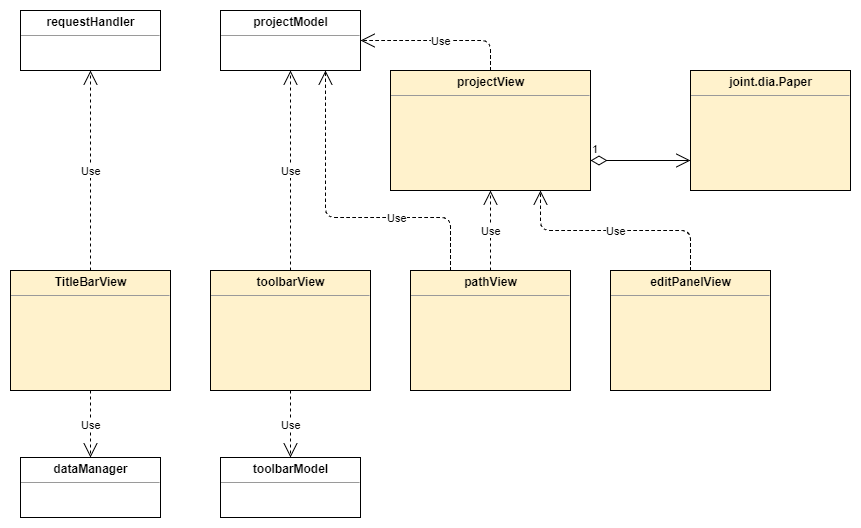
\includegraphics[scale=0.44]{Immagini/DiagrammaArchitettura/View.png}
						\caption{Architettura di View}
					\end{figure}
				Questo package non contiene dei sottopackage.
				Le classi contenute al suo interno verranno elencate qui di seguito.

				\subsubsection{SWEDesigner::Client::View::ProjectView}
					\hypertarget{SWEDesigner::Client::View::ProjectView}{}
					\begin{itemize}
						\item \textbf{Tipo}: \emph{Class};
						\item \textbf{Descrizione}: Questa classe gestisce il diagramma disegnato e le interazioni dell'utente con esso;
						\item \textbf{Padre}: \emph{Backbone.View};
						\item \textbf{Attributi}:
						\begin{itemize}
							\item \emph{model} \\
							Istanza di \hyperlink{SWEDesigner::Model::ProjectModel}{\emph{ProjectModel}} del programma;
							\item \emph{paper} \\
							Oggetto joint.dia.Paper della libreria esterna JointJS;
						\end{itemize}
						\item \textbf{Metodi}:
						\begin{itemize}
							\item \emph{resetSelectedCell(): void} \\
							Pone this.paper.selectedCell a null e genera l'evento "changed-selected-cell";
							\item \emph{mouseMoveFunction(event: JavaScriptEvent): void} \\
							Provoca la traslazione del paper nella direzione del trascinamento del mouse; \\
							Parametri:
							\begin{itemize}
								\item \emph{event: JavaScriptEvent}: Evento;
							\end{itemize}
							\item \emph{blankPointerDown(elem: CellView, event: JavaScriptEvent, x: Double, y: Double): void} \\
							Salva le correnti coordinate al click del mouse nello spazio vuoto del paper; \\
							Parametri:
							\begin{itemize}
								\item \emph{elem: CellView}: Elemento cellView;
								\item \emph{event: JavaScriptEvent}: Evento;
								\item \emph{x: Double}: Coordinata dell'asse delle ascisse;
								\item \emph{y: Double}: Coordinata dell'asse delle ordinate;
							\end{itemize}
							\item \emph{blankPointerUp(elem: CellView, event: JavaScriptEvent, x: Double, y: Double): void} \\
							Elimina le coordinate iniziali al click del mouse nello spazio vuoto del paper; \\
							Parametri:
							\begin{itemize}
								\item \emph{elem: CellView}: Elemento cellView;
								\item \emph{event: JavaScriptEvent}: Evento;
								\item \emph{x: Double}: Coordinata dell'asse delle ascisse;
								\item \emph{y: Double}: Coordinata dell'asse delle ordinate;
							\end{itemize}
							\item \emph{onMouseWheel(elem: CellView, event: JavaScriptEvent): void} \\
							Trasla verticalmente il paper effettuando uno zoom in avanti o indietro a seconda della rotazione della ruota del mouse; \\
							Parametri:
							\begin{itemize}
								\item \emph{elem: CellView}: Elemento cellView;
								\item \emph{event: JavaScriptEvent}: Evento;
							\end{itemize}
							\item \emph{render(): void} \\
							Provoca il render della projectVIew;
							\item \emph{addCell(elem: CellView, event: JavaScriptEvent, x: Double, y: Double): void} \\
							Aggiunge un nuovo elemento al graph chiamando il relativo metodo di \hyperlink{SWEDesigner::Model::ProjectModel}{\emph{ProjectModel}}; \\
							Parametri:
							\begin{itemize}
								\item \emph{elem: cellView}: Elemento CellView;
								\item \emph{event: JavaScriptEvent}: Evento;
								\item \emph{x: Double}: Coordinata dell'asse delle ascisse;
								\item \emph{y: Double}: Coordinata dell'asse delle ordinate;
							\end{itemize}
							\item \emph{deleteCell(event: JavaScriptEvent): void} \\
							Elimina un elemento dal graph chiamando il relativo metodo di ProjectModel;\\
							Parametri:
							\begin{itemize}
								\item \emph{event: JavaScriptEvent}: Evento;
							\end{itemize}
							\item \emph{unembedCell(event: JavaScriptEvent): void} \\
							Rimuove l'innestamento della cella selezionata;\\
							Parametri:
							\begin{itemize}
								\item \emph{event: JavaScriptEvent}: Evento;
							\end{itemize}
							\item \emph{pointerDownFunction(prView: \hyperlink{SWEDesigner::Client::View::projectView}{\emph{projectView}}, elem: cellView, event: JavaScriptEvent, x: double, y: double): void} \\
							Gestice l'evento generato dal click (non rilasciato) del mouse nel paper. Se viene cliccato un elemento, genera a sua volta l'evento "changed-selected-cell" gestito da \hyperlink{SWEDesigner::Client::View::EditPanelView}{\emph{EditPanelView}};\\
							Parametri:
							\begin{itemize}
								\item \emph{prView: \hyperlink{SWEDesigner::Client::View::ProjectView}{\emph{ProjectView}}}: Istanza di ProjectView;
								\item \emph{elem: cellView}: Elemento CellView;
								\item \emph{event: JavaScriptEvent}: Evento;
								\item \emph{x: Double}: Coordinata dell'asse delle ascisse;
								\item \emph{y: Double}: Coordinata dell'asse delle ordinate;
							\end{itemize}
							\item \emph{pointerUpFunction(prView: \hyperlink{SWEDesigner::Client::View::ProjectView}{\emph{ProjectView}}, elem: CellView, event: JavaScriptEvent, x: Double, y: Double): void} \\
							Gestice l'evento generato dal click (al rilascio) del mouse nel paper (rimozione di un elemento, nesting di un elemento in un'altro, collegamento di una relazione tra elementi);\\
							Parametri:
							\begin{itemize}
								\item \emph{prView: \hyperlink{SWEDesigner::Client::View::projectView}{\emph{projectView}}}: Istanza di projectView;
								\item \emph{elem: CellView}: Elemento cellView;
								\item \emph{event: JavaScriptEvent}: Evento;
								\item \emph{x: Double}: Coordinata dell'asse delle ascisse;
								\item \emph{y: Double}: Coordinata dell'asse delle ordinate;
							\end{itemize}
							\item \emph{switchIn(id: String): void} \\
							Gestisce lo switch in profondità (dall'elemento selezionato il cui id è parametro in input) invocando il relativo metodo di \hyperlink{SWEDesigner::Model::ProjectModel}{\emph{ProjectModel}};\\
							Parametri:
							\begin{itemize}
								\item \emph{id: String}: Identificativo dell'elemento;
							\end{itemize}
							\item \emph{switchOut(diagramType: String): void} \\
							Gestisce lo switch verso un diagramma (il cui tipo è parametro in input) antistante da quello corrente invocando il relativo metodo di \hyperlink{SWEDesigner::Model::ProjectModel}{\emph{ProjectModel}}.\\
							Parametri:
							\begin{itemize}
								\item \emph{diagramType: String}: Tipo di diagramma di destinazione;
							\end{itemize}
							\item \emph{deleteOperationAt(ind: Int): void} \\
							Gestisce l'eliminazione di un diagramma delle bubble invocando il relativo metodo di \hyperlink{SWEDesigner::Model::projectModel}{\emph{projectModel}}.\\
							Parametri:
							\begin{itemize}
								\item \emph{ind: Int}: Indice dell'array di operazioni del diagramma delle bubble da eliminare;
							\end{itemize}
						\end{itemize}
						FAN-IN:
						\begin{itemize}
							\item \hyperlink{SWEDesigner::View::PathView}{\emph{PathView}}: gestisce l'interfaccia grafica della barra di indirizzo;
							\item \hyperlink{SWEDesigner::View::EditPanelView}{\emph{EditPanelView}}: gestisce l'interfaccia grafica del pannello di editing.
						\end{itemize}
						FAN-OUT:
						\begin{itemize}
							\item \hyperlink{SWEDesigner::Model::ProjectModel}{\emph{ProjectModel}}: si occupa di gestire la parte logica dell'editor;
							\item joint.dia.Paper: gestisce l'interfaccia grafica dell'area dei diagrammi.
						\end{itemize}
					\end{itemize}
					
				\subsubsection{SWEDesigner::Client::View::TitlebarView}
					\hypertarget{SWEDesigner::Client::View::TitlebarView}{}
					\begin{itemize}
						\item \textbf{Tipo}: \emph{Class};
						\item \textbf{Descrizione}: È il componente del programma che fa la funzione di view per la barra del titolo, dove saranno collocati il menu dell’applicazione e gli shortcut;
						\item \textbf{Padre}: \emph{Backbone.View};
						\item \textbf{Attributi}:
						\begin{itemize}
							\item \emph{el: String} \\
							Il tag HTML popolato dalla Titlebar;
							\item \emph{events: Object} \\
							Gli eventi verificabili nella titlebar;
						\end{itemize}
						\item \textbf{Metodi}:
						\begin{itemize}
							\item \emph{generateJava(event: JavaScriptEvent): void} \\
							Richiede al server di generare il codice in linguaggio Java del progetto correntemente aperto invocando il rispettivo metodo di \hyperlink{SWEDesigner::Model::RequestHandler}{\emph{RequestHandler}}; \\
							Parametri:
							\begin{itemize}
								\item \emph{event: JavaScriptEvent}: Evento;
							\end{itemize}
							\item \emph{generateJavascript(event: JavaScriptEvent): void} \\
							Richiede al server di generare il codice in linguaggio JavaScript del progetto correntemente aperto invocando il rispettivo metodo di \hyperlink{SWEDesigner::Model::RequestHandler}{\emph{RequestHandler}}; \\
							Parametri:
							\begin{itemize}
								\item \emph{event: JavaScriptEvent}: Evento;
							\end{itemize}
							\item \emph{newProject(event: JavaScriptEvent): void} \\
							Crea un nuovo progetto invocando il rispettivo metodo di \hyperlink{SWEDesigner::Model::DataManager}{\emph{DataManager}} \\
							Parametri:
							\begin{itemize}
								\item \emph{event: JavaScriptEvent}: Evento;
							\end{itemize}
							\item \emph{openProject(event: JavaScriptEvent): void} \\
							Apre un progetto invocando il rispettivo metodo di \hyperlink{SWEDesigner::Model::DataManager}{\emph{DataManager}} \\
							Parametri:
							\begin{itemize}
								\item \emph{event: JavaScriptEvent}: Evento;
							\end{itemize}
							\item \emph{saveProject(event: JavaScriptEvent): void} \\
							Salva il progetto correntemente aperto invocando il rispettivo metodo di \hyperlink{SWEDesigner::Model::DataManager}{\emph{DataManager}} \\
							Parametri:
							\begin{itemize}
								\item \emph{event: JavaScriptEvent}: Evento;
							\end{itemize}
							\item \emph{saveProjectAs(event: JavaScriptEvent): void} \\
							Salva il progetto correntemente aperto con nome specificato dall'utente invocando il rispettivo metodo di \hyperlink{SWEDesigner::Model::DataManager}{\emph{DataManager}} \\
							Parametri:
							\begin{itemize}
								\item \emph{event: JavaScriptEvent}: Evento;
							\end{itemize}
						\end{itemize}
						FAN-IN:\\
						Non ci sono dipendenze IN.\\
						FAN-OUT:
						\begin{itemize}
							\item \hyperlink{SWEDesigner::Model::RequestHandler}{\emph{RequestHandler}}: gestisce la comunicazione con il server;
							\item \hyperlink{SWEDesigner::Model::DataManager}{\emph{DataManager}}: gestisce la persistenza dei dati su file system.
						\end{itemize}
					\end{itemize}

				\subsubsection{SWEDesigner::Client::View::ToolbarView}
					\hypertarget{SWEDesigner::Client::View::ToolbarView}{}
					\begin{itemize}
						\item \textbf{Tipo}: \emph{Class};
						\item \textbf{Descrizione}: È il componente del programma che fa la funzione di view per la toolbar dove saranno collocati gli strumenti per editare i diagrammi;
						\item \textbf{Padre}: \emph{Backbone.View};
						\item \textbf{Attributi}:
						\item \textbf{Attributi}:
						\begin{itemize}
							\item \emph{el: String} \\
							Il tag HTML popolato dalla Toolbar;
							\item \emph{events: Object} \\
							Gli eventi verificabili nella Toolbar;
						\end{itemize}
						\item \textbf{Metodi}:
						\begin{itemize}
							\item \emph{addElement(event: JavaScriptEvent): void} \\
							Aggiunge un elemento al diagramma alla selezione di uno strumento invocando il rispettivo metodo di \hyperlink{SWEDesigner::Model::ToolbarModel}{\emph{ToolbarModel}}; \\
							Parametri:
							\begin{itemize}
								\item \emph{event: JavaScriptEvent}: Evento;
							\end{itemize}
							\item \emph{initialize(): void} \\
							Inizializza ToolbarView; 
							\item \emph{render(): void} \\
							Provoca il render della toolbar in base al diagramma correntemente visualizzato; 
						\end{itemize}
						FAN-IN:\\
						Non ci sono dipendenze IN.\\
						FAN-OUT:
						\begin{itemize}
							\item \hyperlink{SWEDesigner::Model::ProjectModel}{\emph{ProjectModel}}: si occupa di gestire la parte logica dell'editor;
							\item \hyperlink{SWEDesigner::Model::ToolbarModel}{\emph{ToolbarModel}}: si occupa di gestire la parte logica della toolbar.
						\end{itemize}
					\end{itemize}

				\subsubsection{SWEDesigner::Client::View::PathView}
					\hypertarget{SWEDesigner::Client::View::PathView}{}
					\begin{itemize}
						\item \textbf{Tipo}: \emph{Class};
						\item \textbf{Descrizione}: È il componente del programma che fa la funzione di view per il cosiddetto breadcrumb dove viene inserita la posizione corrente;
						\item \textbf{Padre}: \emph{Backbone.View};
						\item \textbf{Attributi}:
						\begin{itemize}
							\item \emph{el: String} \\
							Il tag HTML popolato dalla path;
							\item \emph{events: Object} \\
							Gli eventi verificabili nella path;
						\end{itemize}
						\item \textbf{Metodi}:
						\begin{itemize}
							\item \emph{initialize(): void} \\
							Inizializza PathView; 
							\item \emph{render(): void} \\
							Provoca il render del path in base al diagramma correntemente visualizzato; 
							\item \emph{switchDiagram(event: JavaScriptEvent): void} \\
							Metodo chiamato da evento generato. Switch verso un tipo antistante di diagramma.; \\
							Parametri:
							\begin{itemize}
								\item \emph{event: JavaScriptEvent}: Evento;
							\end{itemize}
						\end{itemize}
						FAN-IN:
						Non ci sono dipendenze IN. \\
						FAN-OUT:
						\begin{itemize}
							\item \hyperlink{SWEDesigner::Model::ProjectModel}{\emph{ProjectModel}}: si occupa di gestire la parte logica dell'editor;
							\item \hyperlink{SWEDesigner::View::ProjectView}{\emph{ProjectView}}: si occupa di gestire la parte grafica del model.
						\end{itemize}
					\end{itemize}

				\subsubsection{SWEDesigner::Client::View::EditPanelView}
					\hypertarget{SWEDesigner::Client::View::EditPanelView}{}
					\begin{itemize}
						\item \textbf{Tipo}: \emph{Class};
						\item \textbf{Descrizione}: ;
						\item \textbf{Padre}: \emph{Backbone.View};
						\item \textbf{Attributi}:
						\begin{itemize}
							\item \emph{currentTemplate: Object}\\
							Il template correntemente caricato e renderizzato;
							\item \emph{el: String} \\
							Il tag HTML popolato dalla path;
							\item \emph{events: Object} \\
							Gli eventi verificabili nella path;
							\item \emph{tagname: String} \\
							Il tag HTML popolato dal pannello;
						\end{itemize}
						\item \textbf{Metodi}:
						\begin{itemize}
							\item \emph{confirmEdit(event: JavaScriptEvent): void} \\
							Metodo chiamato da evento generato, salva le modifiche apportate ad una proprietà del contenuto selezionato nel pannello; \\
							Parametri:
							\begin{itemize}
								\item \emph{event: JavaScriptEvent}: Evento;
							\end{itemize}
							\item \emph{execCommand(event: JavaScriptEvent): void} \\
							Metodo chiamato da evento generato, esegue il metodo definito dal nome dell'elemento generante l'evento sul contenuto selezionato nel pannello; \\
							Parametri:
							\begin{itemize}
								\item \emph{event: JavaScriptEvent}: Evento;
							\end{itemize}
							\item \emph{initialize(): void} \\
							Inizializza la EditPanelView; 
							\item \emph{render(): void} \\
							Provoca il render del pannello in base all'elemento del paper cliccato; 
							\item \emph{reset(): void} \\
							Provoca il reset del pannello; 
							\item \emph{saveCode(event: JavaScriptEvent): void} \\
							Metodo chiamato da evento generato, salva il codice interno ad una customBubble; \\
							Parametri:
							\begin{itemize}
								\item \emph{event: JavaScriptEvent}: Evento;
							\end{itemize}
							\item \emph{switch(event: JavaScriptEvent): void} \\
							Metodo chiamato da evento generato, esegue lo switch in profondità del tipo di diagramma; \\
							Parametri:
							\begin{itemize}
								\item \emph{event: JavaScriptEvent}: Evento;
							\end{itemize}
							\item \emph{switchDiagram(event: JavaScriptEvent): void} \\
							Metodo chiamato da evento generato, esegue lo switch verso un tipo antistante di diagramma; \\
							Parametri:
							\begin{itemize}
								\item \emph{event: JavaScriptEvent}: Evento;
							\end{itemize}
							\item \emph{unembedCell(event: JavaScriptEvent): void} \\
							Metodo chiamato da evento generato, rimuove la bubble selezionata nel pannello dall'innesto; \\
							Parametri:
							\begin{itemize}
								\item \emph{event: JavaScriptEvent}: Evento;
							\end{itemize}
						\end{itemize}
						FAN-IN:\\
						Non ci sono dipendenze IN. \\
						FAN-OUT:
						\begin{itemize}
							\item \hyperlink{SWEDesigner::View::ProjectView}{\emph{ProjectView}}: si occupa di gestire la parte grafica del model.
						\end{itemize}
					\end{itemize}

			\subsection{SWEDesigner::Server}
				% IMMAGINE ARCHITETTURA SERVER GENERALE
				\begin{figure}[H]\label{fig:ServerSubsystem}
					\centering
					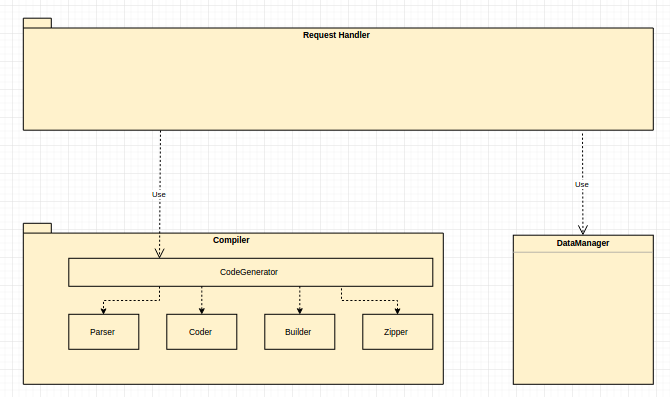
\includegraphics[scale=0.4]{Immagini/DiagrammaArchitettura/ServerSubsystem.png}
					\caption{Architettura del server}
				\end{figure}
				I package contenuti al suo interno sono:
				\begin{itemize}
					\item SWEDesigner::Server::CodeGenerator;
					\item SWEDesigner::Server::DAORequestHandler;
					\item SWEDesigner::Server::RequestHandler.
				\end{itemize}
				Questo package non contiene delle classi.

			\subsection{SWEDesigner::Server::CodeGenerator}
				I package contenuti al suo interno sono:
				\begin{itemize}
					\item SWEDesigner::Server::CodeGenerator::Builder;
					\item SWEDesigner::Server::CodeGenerator::Coder;
					\item SWEDesigner::Server::CodeGenerator::Parser;
					\item SWEDesigner::Server::CodeGenerator::Zipper.
				\end{itemize}
				Le classi contenute al suo interno verranno elencate qui di seguito.

				\subsubsection{SWEDesigner::Server::CodeGenerator::CodeGenerator}
				\hypertarget{SWEDesigner::Server::CodeGenerator::CodeGenerator}
				E' il componente che rende disponibile la funzionalità per cui, dato un file valido in formato JSON, restituisce un pacchetto in formato .zip contenente i file del codice sorgente che costituiscono il programma rappresentato dal file in input. I file prodotti sono strutturati in packages, come indicato nel file JSON in input.\\
					FAN-IN:
					\begin{itemize}
						\item Server::RequestHandler::Receiver: si occupa di gestire le comunicazioni in entrata dal client.
					\end{itemize}
					FAN-OUT:
					\begin{itemize}
						\item Server::RequestHandler::Sender: si occupa di gestire le comunicazioni in uscita verso il client;
						\item Parser: si occupa di creare un oggetto che contiene le informazioni ricevute in input;
						\item Coder: si occupa della traduzione in codice dell'oggetto ottenuto dal Parser;
						\item Builder: si occupa di organizzare in maniera organica il codice generato dal Coder;
						\item Zipper: si occupa di creare un archivio .zip contenente in codici sorgente precedentemente creati.
					\end{itemize}

			\subsection{SWEDesigner::Server::CodeGenerator::Builder}
				Questo package non contiene dei sottopackage.\\
				Le classi contenute al suo interno verranno elencate qui di seguito.
				\subsubsection{SWEDesigner::Server::CodeGenerator::Builder::Builder}
				È il componente che rende disponibile la funzionalità, dato un file JSON in input che rappresenti un programma, di ottenere un oggetto contenitore del codice sorgente corrispondente al contenuto del file di input. Tale codice è suddiviso e strutturato come indicato nel file di input.\\
					FAN-IN:
					\begin{itemize}
						\item Zipper: si occupa di creare un archivio .zip contenente in codici sorgente precedentemente creati.
					\end{itemize}
					FAN-OUT:
					\begin{itemize}
						\item Coder: componente che funge da interfaccia alle operazioni di codifica di una stringa permettendo quindi di trasformare le informazioni del file in formato JSON in codice sorgente.
					\end{itemize}

			\subsection{SWEDesigner::Server::CodeGenerator::Coder}
				% IMMAGINE ARCHITETTURA CODER
				\begin{figure}[H]\label{fig:Coder}
					\centering
					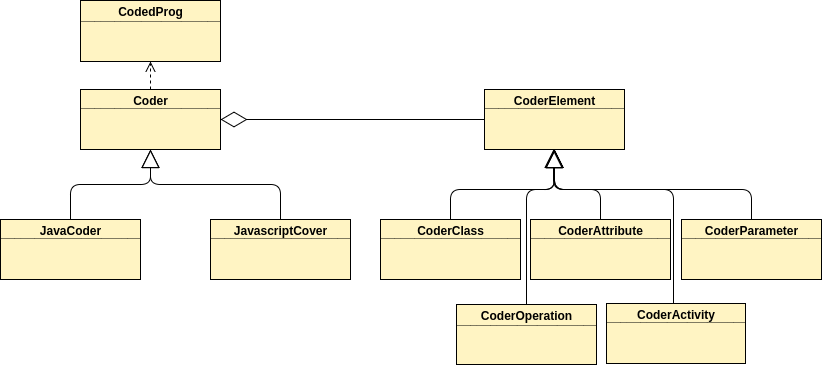
\includegraphics[scale=0.46]{Immagini/DiagrammaArchitettura/Coder.png}
					\caption{Architettura di Coder}
				\end{figure}

				Questo package non contiene dei sottopackage.\\
				Le classi contenute al suo interno verranno elencate qui di seguito.
				\subsubsection{SWEDesigner::Server::CodeGenerator::Coder::Coder}
				Componente che funge da interfaccia alle operazioni di codifica di una stringa, in formato JSON che rappresenta un programma valido; tali operazioni permettono di ottenere un oggetto contenente il codice sorgente, in Java o Javascript, corrispondente alla stringa in input.\\
					FAN-IN:
					\begin{itemize}
						\item JavaCoder: si occupa di trasformare un oggetto JSON ricevuto in input in un oggetto contenente il codice sorgente scritto in java;
						\item JavaScriptCoder: si occupa di trasformare un oggetto JSON ricevuto in input in un oggetto contenente il codice sorgente scritto in javascript.
					\end{itemize}
					FAN-OUT:
					\begin{itemize}
						\item CodedProg: componente che contiene il codice prodotto dal Coder;
						\item CoderElement: componente astratto che offre la funzionalità che permette di associare ad ogni stringa contenuta nel file JSON il corrispondente codice sorgente.
					\end{itemize}

				\subsubsection{SWEDesigner::Server::CodeGenerator::Coder::JavaCoder}
				È il componente che rende disponibile la funzionalità, dato un oggetto in input che rappresenta un file JSON parsificato, di ottenere un oggetto contenente il codice sorgente, in linguaggio Java, corrispondente all'oggetto in input.\\
					Non ci sono dipendenze IN.\\
					FAN-OUT:
					\begin{itemize}
						\item Coder: componente che funge da interfaccia alle operazioni di codifica di una stringa permettendo quindi di trasformare le informazioni del file in formato JSON in codice sorgente.
					\end{itemize}

				\subsubsection{SWEDesigner::Server::CodeGenerator::Coder::JavascriptCoder}
				È il componente che rende disponibile la funzionalità, dato un oggetto in input che rappresenta un file JSON parsificato, di ottenere un oggetto contenente il codice sorgente, in linguaggio Javascript, corrispondente all'oggetto in input.\\
					Non ci sono dipendenze IN.\\
					FAN-OUT:
					\begin{itemize}
						\item Coder: componente che funge da interfaccia alle operazioni di codifica di una stringa permettendo quindi di trasformare le informazioni del file in formato JSON in codice sorgente.
					\end{itemize}

				\subsubsection{SWEDesigner::Server::CodeGenerator::Coder::CoderClass}
				È il componente che mette a disposizione la funzionalità, data una stringa in input in formato JSON che rappresenta una classe valida, di ottenere il corrispondente codice sorgente di tale classe.\\
					Non ci sono dipendenze IN.\\
					FAN-OUT:
					\begin{itemize}
						\item CoderElement: componente astratto che offre la funzionalità che permette di associare ad ogni stringa contenuta nel file JSON il corrispondente codice sorgente.
					\end{itemize}

				\subsubsection{SWEDesigner::Server::CodeGenerator::Coder::CoderOperation}
				È il componente che mette a disposizione la funzionalità, data una stringa in input in formato JSON che rappresenta un'operazione valida, di ottenere il corrispondente codice sorgente di tale operazione.\\
					Non ci sono dipendenze IN.\\
					FAN-OUT:
					\begin{itemize}
						\item CoderElement: componente astratto che offre la funzionalità che permette di associare ad ogni stringa contenuta nel file JSON il corrispondente codice sorgente.
					\end{itemize}

				\subsubsection{SWEDesigner::Server::CodeGenerator::Coder::CoderParameter}
				È il componente che mette a disposizione la funzionalità, data una stringa in input in formato JSON che rappresenta un parametro di una lista valido, di ottenere il corrispondente codice sorgente di tale parametro. È possibile scegliere fra la codifica in Java o Javascript.\\
					Non ci sono dipendenze IN.\\
					FAN-OUT:
					\begin{itemize}
						\item CoderElement: componente astratto che offre la funzionalità che permette di associare ad ogni stringa contenuta nel file JSON il corrispondente codice sorgente.
					\end{itemize}

				\subsubsection{SWEDesigner::Server::CodeGenerator::Coder::CoderAttribute}
				È il componente che mette a disposizione la funzionalità, data una stringa in input in formato JSON che rappresenta un attributo valido, di ottenere il corrispondente codice sorgente di tale attributo. È possibile scegliere fra la codifica in Java o Javascript.\\
				Non ci sono dipendenze IN.\\
					FAN-OUT:
					\begin{itemize}
						\item CoderElement: componente astratto che offre la funzionalità che permette di associare ad ogni stringa contenuta nel file JSON il corrispondente codice sorgente.
					\end{itemize}

				\subsubsection{SWEDesigner::Server::CodeGenerator::Coder::CoderActivity}
				È il componente che mette a disposizione la funzionalità, data una stringa in input in formato JSON che rappresenta un diagramma delle attività valido, di ottenere il corrispondente codice sorgente di tale attività. È possibile scegliere fra la codifica in Java o Javascript.\\
					Non ci sono dipendenze IN.\\
					FAN-OUT:
					\begin{itemize}
						\item CoderElement: componente astratto che offre la funzionalità che permette di associare ad ogni stringa contenuta nel file JSON il corrispondente codice sorgente;
						\item DAO: si occupa di gestire il database delle bubble.
					\end{itemize}

				\subsubsection{SWEDesigner::Server::CodeGenerator::Coder::CodedProg}
				È il componente che contiene il codice sorgente prodotto dal Coder.\\
					FAN-IN:
					\begin{itemize}
						\item Coder: componente che funge da interfaccia alle operazioni di codifica di una stringa permettendo quindi di trasformare le informazioni del file in formato JSON in codice sorgente.
					\end{itemize}
					Non ci sono dipendenze OUT.
				
				\subsubsection{SWEDesigner::Server::CodeGenerator::Coder::CoderElement}
				Componente astratta che offre la funzionalità di ottenere, data una stringa in input in formato JSON che rappresenta un elemento di classe valido, il corrispondente codice sorgente, in Java o Javascript.\\
					FAN-IN:
					\begin{itemize}
						\item Coder: componente che funge da interfaccia alle operazioni di codifica di una stringa permettendo quindi di trasformare le informazioni del file in formato JSON in codice sorgente;
						\item CoderClass: componente che permette data una stringa in input in formato JSON che rappresenta un diagramma delle classi valido, di ottenere il corrispondente codice sorgente di tale classe;
						\item CoderOperations: componente che permette data una stringa in input in formato JSON che rappresenta un'operazione valida, di ottenere il corrispondente codice sorgente di tale operazione;
						\item CoderAttributes: componente che permette data una stringa in input in formato JSON che rappresenta un attributo valido, di ottenere il corrispondente codice sorgente di tale attributo;
						\item CoderActivity: componente che permette data una stringa in input in formato JSON che rappresenta un diagramma delle attività valido, di ottenere il corrispondente codice sorgente di tale attività;
						\item CoderParameter: componente che permette data una stringa in input in formato JSON che rappresenta un parametro valido, di ottenere il corrispondente codice sorgente di tale parametro.
					\end{itemize}
					Non ci sono dipendenze OUT.

			\subsection{SWEDesigner::Server::CodeGenerator::Parser}
				Questo package non contiene dei sottopackage.
				Le classi contenute al suo interno verranno elencate qui di seguito.
				\subsubsection{SWEDesigner::Server::CodeGenerator::Parser::Parser}
				È il componente che rende disponibile la funzionalità, dato un file JSON valido in input, di ottenere un oggetto contenente le informazioni che costituiscono il file in input.\\
					FAN-IN:
					\begin{itemize}
						\item CodeGenerator: si occupa di restituire in output un archivio zip contenente i codici sorgenti generati a partire dal file JSON ricevuto in input;
						\item Coder: componente che funge da interfaccia alle operazioni di codifica di una stringa permettendo quindi di trasformare le informazioni del file in formato JSON in codice sorgente.
					\end{itemize}
					Non ci sono dipendenze OUT.

			\subsection{SWEDesigner::Server::CodeGenerator::Zipper}
				Questo package non contiene dei sottopackage.\\
				Le classi contenute al suo interno verranno elencate qui di seguito.
				\subsubsection{SWEDesigner::Server::CodeGenerator::Zipper::Zipper}
				E' il componente che rende disponibile la funzionalità per cui, dato un file valido in formato JSON, restituisce un pacchetto in formato .zip contenente i file del codice sorgente che costituiscono il programma rappresentato dal file in input. I file prodotti sono strutturati in packages, come indicato nel file JSON in input.\\
					FAN-IN:
					\begin{itemize}
						\item CodeGenerator: si occupa di restituire in output un archivio zip contenente i codici sorgenti generati a partire dal file JSON ricevuto in input.
					\end{itemize}
					FAN-OUT:
					\begin{itemize}
						\item Builder: componente che si occupa di creare un oggetto contenitore con il codice sorgente, partendo dalle informazioni prese dal file JSON ricevuto in input che rappresenta un programma.
					\end{itemize}

				\subsubsection{SWEDesigner::Server::DAO}
				\hypertarget{SWEDesigner::Server::DAO}
				Questa classe si occupa di gestire il database delle bubble.\\
					FAN-IN:
					\begin{itemize}
						\item Coder: componente che funge da interfaccia alle operazioni di codifica di una stringa permettendo quindi di trasformare le informazioni del file in formato JSON in codice sorgente.
					\end{itemize}
					Non ci sono dipendenze OUT.

			\subsection{SWEDesigner::Server::RequestHandler}
				\hypertarget{SWEDesigner::Server::RequestHandler}
				Questo package non contiene dei sottopackage.\\
				Le classi contenute al suo interno verranno elencate qui di seguito.
				\subsubsection{SWEDesigner::Server::RequestHandler::Sender}
				Si occupa di gestire le comunicazioni in uscita verso il client.\\
					FAN-IN:
					\begin{itemize}
						\item CodeGenerator: si occupa di restituire in output un archivio zip contenente i codici sorgenti generati a partire dal file JSON ricevuto in input.
					\end{itemize}
					FAN-OUT:
					\begin{itemize}
						\item Client::Model::RequestHandler::Receiver: si occupa di gestire le comunicazioni in entrata dal server.
					\end{itemize}
					
				\subsubsection{SWEDesigner::Server::RequestHandler::Receiver}
				Si occupa di gestire le comunicazioni in entrata dal client.\\
					FAN-IN:
					\begin{itemize}
						\item Client::Model::RequestHandler::Sender: si occupa di gestire le comunicazioni in uscita verso il server.
					\end{itemize}
					FAN-OUT:
					\begin{itemize}
						\item CodeGenerator: si occupa di restituire in output un archivio zip contenente i codici sorgenti generati a partire dal file JSON ricevuto in input.
					\end{itemize}
\end{document}
